\documentclass[11pt]{article}

\usepackage{graphicx}

\usepackage[margin=0.8in]{geometry}

\title{\vspace{-2cm}Dynamics in an uni-directional billiard}

\author{Martin Horvat}

\date{November, 2009}

\begin{document}
\maketitle

Dynamics in a billiard with inner and outer boundary parallel to each other. In such a billiard the dynamics is unidirectional. The inner boundary is defined in Cartesian coordinates as
%
$$
  r(\phi) (\cos(\phi), \sin(\phi))
$$
%
and the outer boundary is given as
%
$$ 
r(\phi) (\cos(\phi), \sin(\phi)) +d\,n(\phi) 
$$
%
where d is the width of the billiard and $n(\phi)$ is the normal vector to the boundaries at the angle $\phi$
%
$$
n(\phi) = (r'(\phi)\sin(\phi) + r(\phi)\cos(\phi),-r'(\phi)\cos(\phi) + r(\phi)\sin(\phi))/\sqrt{r'(\phi)^2+r^2(\phi)}
$$
%
Here we define the $r(\phi)$ via trigonometrical series
%
$$
r(\phi) = a_0 + \sum_{n=1}^\infty a_n \cos(n \phi) + b_n \sin(n \phi)
$$
%
This series can be more sophistically written as
%
$$
r(\phi) = \sum_{s \in \{0,1\}} \sum_{n=0}^\infty c_{s,n} f(s,n \phi)
$$
%
with $f(0,x) = \sin(x)$ and $f(1,x)=\cos(x)$. The present "software package" brings two programs written in C/C++: \verb|bill|, \verb|calc|. The last, "calc", is command line program with inputs via command line and standard input (stdin), and the first "bill" (short for billiard) is basically the second program "calc" with GUI (Graphical User Inferface) created with GLADE. The latter need the file "bill.glade" which contains the information about the GUI in an XML form.
%
\begin{figure}[!htb]
\centering
(a)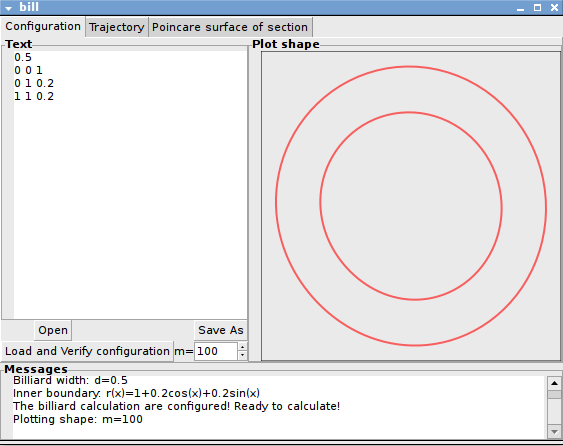
\includegraphics[width=5cm]{screen1.png}
(b)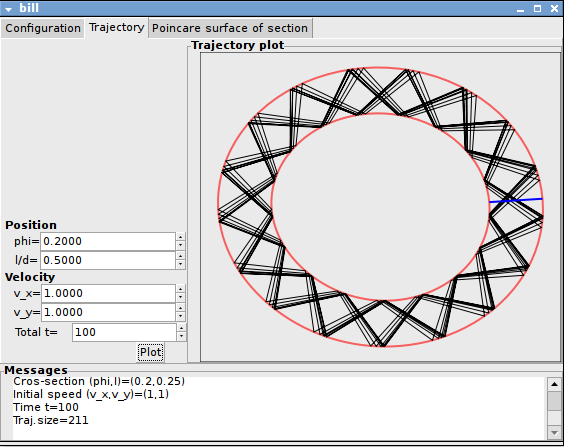
\includegraphics[width=5cm]{screen2.png}
(c)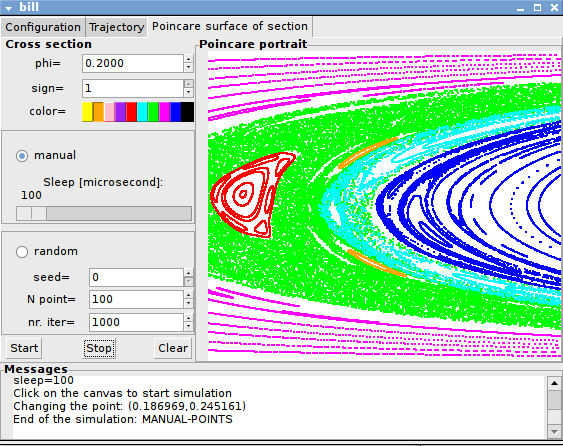
\includegraphics[width=5cm]{screen3.png}
\caption{Screenshots of the program "bill" using the billiard with $r(x)=1+0.2\cos(x)+0.2\sin(x)$: (a) configuration, (b) trajectory calculation,
(c) phase-space portrait. }
\end{figure}

The source and the program you can get here \verb|linux|, which is portable to M\$ Windows by using GTK for Win32 and Dev++. The binaries and required GTK library and .dll files by the program are in \verb|win|.

\end{document}
